\chapter{Desarrollo}\label{ch:chapter_4}


\section{Diseño del sistema}

En la figura~\ref{fig:chapter_1.overview} vimos un esquema general del sistema, el cual recibe documentos en formato
PDF y genera objetos que contienen la información más importante de los mismos.
En la figura~\ref{fig:chapter_1.specific} vimos que se va a incluir también el desarollo de dos interfaces, una web
y una de línea de comandos.

En la figura~\ref{fig:chapter_4.overview} vemos que el sistema tiene dos componentes principales: el \textit{Reader}
y el \textit{Generator}

\begin{figure}
    \begin{center}
        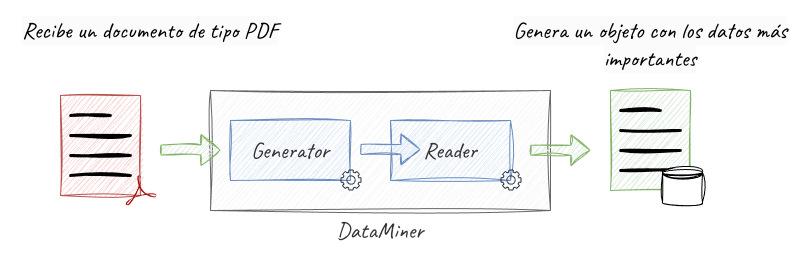
\includegraphics[width=\textwidth]{./chapter/4/images/chapter_4.overview}
        \caption{Esquema de los componentes principales}
        \label{fig:chapter_4.overview}
    \end{center}
\end{figure}

\subsection*{Componente \textit{Generator}}

Este componente sirve como el motor inicial en el proceso, encargado de convertir documentos de cualquier formato a
texto plano.

Se compone de tres conjuntos de elementos y un orquestador al que llamaremos \textit{Engine} responsable de la
coordinación de las operaciones.

Diagrama UML del componente generator.

\subsubsection*{Preprocesadores}
Los preprocesadores preparan el documento original para facilitar su conversión a texto.
En esta implementación no se ha desarrollado ningún preprocesador.

Comunicación del Engine con los preprocesadores definidos.


\subsubsection*{Procesadores}
Actúan como el núcleo del Generator, donde se realiza la conversión efectiva del documento a texto. Funcionan mediante
un sistema competitivo donde varios procesadores evalúan su propia aptitud para manejar el documento en cuestión,
seleccionando el más adecuado para llevar a cabo la tarea.

Este enfoque modular y competitivo asegura que el procesamiento del texto sea no solo eficiente, sino también
extremadamente flexible, adaptándose a las variaciones en la naturaleza de los documentos procesados.


Comunicación del Engine con los procesadores definidos.

En la actual implementación, hemos desarrollado un único procesador especializado en transformar documentos PDF a
texto. Este procesador utiliza la utilidad de línea de comandos `pdftotext` para llevar a cabo la conversión (Glyph \&
Cog, 2023).

\subsubsection*{Postprocesadores}
Estos componentes perfeccionan el texto generado, eliminando errores como caracteres no UTF-8 y espacios en blanco
innecesarios, lo que mejora significativamente la calidad del texto resultante. En esta implementación, se han
desarrollado varios post-procesadores:

\begin{itemize}
    \item
    Word Limit PostProcessor: Se detectó que los elementos de interés, como nombres, documentos de identidad y fechas de
    contratos, típicamente aparecen en las primeras páginas. Este procesador limita el análisis a las primeras N
    palabras del documento.
    \item UTF8 PostProcessor: Implementado tras detectar caracteres no UTF-8 en algunos documentos, este post-procesador
    elimina dichos caracteres.
    \item Character Replace PostProcessor: Desarrollado para eliminar caracteres específicos que complicaba las pruebas.
\end{itemize}

\subsubsection*{Engine}
Este es el orquestador del componente, encargado de hacer las llamadas a los demás elementos registrados en la
aplicación. Coordina el flujo entre los pre-procesadores, procesadores y post-procesadores para asegurar que el
documento sea procesado de manera correcta.

\subsection*{Reader}
El componente Reader juega un papel crucial en el proceso de interpretación y procesamiento del texto plano obtenido a
partir de la salida del componente Generator anterior..

Funciona mediante un sistema de procesadores organizados en una única capa, que opera bajo un mecanismo competitivo
similar al del componente Generator. En este sistema, los procesadores compiten entre sí para determinar cuál es el más
adecuado para analizar y extraer la información estructurada necesaria del texto.

Diagrama UML del componente Reader.

\subsubsection*{Procesadores}
Cada uno de estos procesadores es invocado secuencialmente para evaluar su idoneidad en el manejo del documento
específico..

Una vez seleccionado, el procesador elegido procede a ejecutar una serie de tareas que incluyen la identificación y
extracción de entidades clave. En esta implementación, se han desarrollado los siguientes procesadores:

\begin{itemize}
    \item Residential Lease Processor: Evalúa si el documento se trata de un contrato de alquiler de vivienda entre
    particulares. En caso afirmativo, extrae la información más relevante del mismo, como los nombres de los
    arrendadores, los arrendatarios y la fecha del contrato.
    \item Vehicle Sale And Purchase Processor: Evalúa si el documento se trata de un contrato de compraventa de
    vehículos
    entre particulares. En caso afirmativo, extrae la información más relevante del mismo, como los nombres de los
    compradores y vendedores y la fecha de la transacción.
\end{itemize}

\subsubsection*{Engine}
Este es el orquestador del componente, encargado de hacer las llamadas a los demás elementos registrados en la
aplicación, en este caso únicamente los procesadores.


\section{Tecnologías utilizadas}

A continuación, se describen las principales tecnologías utilizadas en el proyecto, categorizadas en distintas áreas
según su propósito y aplicación.

\subsection*{Backend}

*PHP

Es un lenguaje de scripting de propósito general que está especialmente diseñado para el desarrollo web.
PHP permite crear aplicaciones web dinámicas y está ampliamente soportado en servidores web.

Symfony

Symfony es un framework PHP ampliamente utilizado para desarrollar aplicaciones web.
Ofrece una arquitectura robusta y flexible, que facilita el desarrollo de aplicaciones mantenibles y escalables.

Twig

Twig es un motor de plantillas para PHP, utilizado principalmente en proyectos basados en
Symfony.
Facilita la creación de vistas dinámicas y mantenibles, separando la lógica de presentación del código de negocio.

\subsection*{Frontend}

HTML5

Es el estándar de marcado para crear páginas web.
HTML5 introduce nuevas funcionalidades como elementos semánticos y multimedia, mejorando la accesibilidad y la
interoperabilidad de las páginas web.

CSS3

Es la tecnología de estilos para el diseño visual.
CSS3 permite aplicar estilos complejos y responsivos a los elementos HTML, mejorando la presentación y la experiencia
del usuario.

JavaScript

Es el lenguaje de programación para la interactividad del lado del cliente.
JavaScript permite crear experiencias de usuario dinámicas y responsivas, manejando eventos y actualizando el contenido
de la página sin recargar.

Bootstrap

Es un framework de front-end que facilita el diseño de sitios y aplicaciones web
responsivas y móviles.
Bootstrap proporciona una colección de componentes CSS
y JavaScript predefinidos que aceleran el desarrollo de interfaces de usuario atractivas.

Font Awesome

Es una biblioteca de iconos vectoriales y herramientas que proporciona una amplia gama de
iconos escalables y personalizables para su uso en proyectos web.
Facilita la inclusión de iconos de alta calidad sin depender de imágenes.

\subsection*{Gestión de dependencias}

Composer

Es una herramienta de gestión de dependencias para PHP, que
permite declarar las bibliotecas de las que depende tu proyecto
y las gestiona.
Composer asegura que las versiones correctas de las bibliotecas se instalen y mantengan actualizadas.

\subsection*{Control de versiones}

Git

Es un sistema de control de versiones distribuido, diseñado para manejar todo, desde proyectos
pequeños hasta muy grandes con rapidez y eficiencia.
Git permite a los desarrolladores colaborar de manera efectiva, rastreando cambios y gestionando ramas y fusiones.


GitHub

GitHub es una plataforma de hospedaje de repositorios Git.
Proporciona herramientas para la colaboración, la revisión de código y la gestión de proyectos, facilitando el trabajo
en equipo y la integración continua.

\subsection*{Automatización}

Make

Make es una herramienta de automatización de tareas que utiliza archivos Makefile para definir y ejecutar tareas de
construcción y gestión de proyectos.
Facilita la automatización de tareas repetitivas y la configuración del entorno de desarrollo.

\subsection*{Pruebas}

PHPUnit

PHPUnit es un marco de pruebas unitarias para PHP. Permite a los desarrolladores escribir y ejecutar pruebas
automatizadas
para asegurar que el código se comporta como se espera, facilitando el desarrollo de software de alta calidad.

GitHub Actions

Es una plataforma de integración continua que permite automatizar flujos de trabajo directamente desde GitHub.
GitHub Actions facilita la configuración de pipelines de CI/CD, ejecutando pruebas y despliegues automáticamente con
cada cambio en el repositorio.

\subsection*{Contenerización}

Docker

Docker es una plataforma que permite desarrollar, enviar y ejecutar aplicaciones dentro de
contenedores.
Proporciona un entorno consistente para el desarrollo, pruebas y despliegue, asegurando que las aplicaciones funcionen
de manera idéntica en diferentes entornos.

Docker Compose

Docker Compose es una herramienta para definir y ejecutar aplicaciones Docker multi-contenedor.
Permite orquestar varios servicios que componen una aplicación, facilitando
la configuración y gestión de entornos de desarrollo complejos.

\subsection*{Logs}

Monolog

Monolog es una biblioteca de logging para PHP. Permite enviar registros a varios destinos, como archivos, bases de datos
y servicios de terceros, facilitando la monitorización y depuración de aplicaciones.

Elastic Search

Elasticsearch es un motor de búsqueda y análisis de texto completo basado en Lucene.
Permite almacenar, buscar y analizar grandes volúmenes de datos en tiempo real.

Logstash

Logstash es una herramienta de procesamiento de datos que ingesta, transforma y envía datos a varios
destinos.
Es parte del paquete Elasticsearch, Logstash, Kibana (ELK) y facilita la recolección y procesamiento de logs.

Kibana

Kibana es una herramienta de visualización de datos que trabaja en conjunto con Elasticsearch.
Permite a los usuarios crear gráficos y dashboards interactivos para visualizar y analizar los datos de logs almacenados
en Elasticsearch.

\subsection*{Componente Generator}

Pdf to text

Pdf to Text es una herramienta que convierte documentos PDF en texto plano.
Permite extraer el contenido textual de archivos PDF, lo cual es útil para la posterior manipulación y análisis de
datos.

\subsection*{Componente Reader}

Symfony HttpClient

Symfony HttpClient es un cliente HTTP flexible y eficiente para PHP. Permite realizar solicitudes HTTP a servicios
externos, manejar respuestas y gestionar errores de manera sencilla y eficaz.

Symfony Cache

Symfony Cache es un componente de Symfony que proporciona una implementación robusta y flexible para el almacenamiento
en caché.
Permite mejorar el rendimiento de la aplicación mediante el almacenamiento temporal de datos, reduciendo la carga en los
recursos externos.

API Open AI

La API de OpenAI proporciona acceso a modelos avanzados de procesamiento de lenguaje natural.
Permite integrar capacidades de IA en la aplicación, como la generación de texto y el análisis de datos, mejorando las
funcionalidades y experiencias del usuario.


\colorbox{color_highlight}{@TODO: @marlene:}
En cuanto a los datos, los generaste manual. No hay forma de generar datos sintéticos? Se podrían generar 100 o 1000
documentos? Sino, hay que justificarlo bien.

\colorbox{color_highlight}{@TODO: @marlene:}
Vale, veo que si usas el LLM de chatgpt. Eso es algo que no me había quedado claro de la memoria. Sin embargo, aún no
tengo del todo claro qué generas a partir del PDF que recibes. Puedes ejecutar tu herramienta con un contrato? Estás
usando el LLM para extraer los datos del contenido del PDF? Otra pregunta, qué modelo de chatgpt estás usando? Y puedes
mandar el prompt que usaste?


\section{Arquitectura del sistema}

\section*{Pruebas}
Las pruebas en este proyecto son fundamentales para asegurar que la tecnología funciona conforme a las expectativas y
requisitos establecidos. Para garantizar una validación exhaustiva y precisa, se ha diseñado cuidadosamente un sistema
de pruebas descrito a continuación.

\subsection*{Construcción del conjunto de datos de prueba}

\colorbox{color_highlight}{@TODO: @marlene:} menciona el tamaño del dataset
El proceso para encontrar un conjunto de datos de prueba fue complejo, ya que no se encontraron conjuntos de datos de
fuentes abiertas que cumplieran con los requisitos necesarios..

La mayoría de estos conjuntos se distribuyen anonimizados, y nuestra tecnología necesita identificar y extraer
principalmente datos de carácter personal, como nombres, documentos de identidad, direcciones, fechas, importes, números
de cuentas bancarias, entre otros.

Finalmente, se construyó manualmente un conjunto de datos de prueba utilizando modelos de documentos encontrados en
internet, así como contratos reales a los que tuvimos acceso..

Este conjunto de datos se compone de tres subconjuntos:


INSERTAR TABLA

El siguiente paso fue modificar todos los documentos para que todos los datos de carácter personal fueran aleatorios y
no correspondiera a personas reales. Este proceso aseguró la privacidad y cumplió con las normativa de protección de
datos.

Para facilitar la modificación y manejo de estos documentos, se guardaron en formato Markdown, lo que permitió una
edición más rápida en el propio editor de código.

Dado que la entrada del sistema acepta documentos en formato PDF, se desarrolló un pequeño script para convertir cada
documento Markdown en PDF. Este script utiliza plantillas LaTeX para introducir variabilidad en el formato de los
documentos, asegurando una mayor robustez en las pruebas del sistema.


Este enfoque en la creación del conjunto de datos de prueba garantiza que el sistema pueda ser evaluado de manera
exhaustiva y precisa, cubriendo diversos escenarios y tipos de documentos relevantes para la tecnología desarrollada.

\subsection*{Pruebas automáticas}
Las pruebas automáticas son esenciales para garantizar la calidad y la robustez del software. Permiten verificar que el
código se comporta como se espera, identificar errores de manera temprana y asegurar que las nuevas funcionalidades no
introduzcan fallos en el sistema existente..

En este proyecto, se han implementado varios tipos de pruebas automáticas, cada una con un enfoque diferente para cubrir
todas las facetas del desarrollo y la implementación del software.

\subsubsection*{Pruebas unitarias}
Las pruebas unitarias se centran en verificar la funcionalidad de componentes individuales del sistema, como funciones o
métodos. Estas pruebas son cruciales para asegurar que cada parte del código funciona correctamente en aislamiento.

Se utilizan frameworks de pruebas, como PHPUnit, para automatizar estas pruebas y hacerlas repetibles y confiables.


Pruebas unitarias ejecutadas desde un entorno de desarrollo integrado

\subsubsection*{Pruebas funcionales}
Las pruebas funcionales evalúan el sistema desde el punto de vista del usuario final, verificando que las
funcionalidades del software se comportan como se espera cuando se integran varios componentes.


Pruebas funcionales ejecutadas desde la línea de comandos

\subsection*{Integración continua}
La integración continua es una práctica esencial en el desarrollo de software moderno, que implica la integración
frecuente del trabajo de los desarrolladores en un repositorio compartido, normalmente programando la ejecución
automática de los test en un servidor de integración continua, cada vez que se añade un commit al repositorio.

En este proyecto, hemos implementado la integración continua utilizando GitHub Actions, un servicio de automatización
que permite crear flujos de trabajo personalizados para compilar, probar y desplegar código directamente desde GitHub.


Pruebas de Integración continua realizada en GitHub actions.

\section*{Interfaces de usuario}
Aunque el objetivo principal de este trabajo es desarrollar una tecnología, flexible, extensible y que pueda ser
fácilmente integrada en otros sistemas, se han implementado dos tipos de interfaces sencillas, que permiten demostrar el
correcto funcionamiento de la tecnología.

\subsection*{Interfaz de línea de comandos}
La interfaz de línea de comandos es una herramienta para desarrolladores y administradores del sistema. Permite ejecutar
comandos y scripts de manera directa, facilitando la automatización de tareas y la integración con otros sistemas.


Ejecución de la aplicación a través de la línea de comandos

Esta interfaz recibe como parámetro la ruta de un fichero que se pretende analizar y una vez analizado muestra una
representación en formato tabla de la información extraída del mismo.

\subsection*{Interfaz web}
La interfaz web es el principal punto de interacción para la mayoría de los usuarios. Está diseñada para ser intuitiva,
accesible y eficiente, permitiendo a los usuarios realizar una amplia gama de operaciones a través de un navegador web.

Para este proyecto hemos desarrollado una interfaz con las siguientes características

\begin{itemize}
    \item
    Diseño Responsive: La interfaz web está diseñada para ser accesible desde dispositivos de escritorio y móviles,
    asegurando una experiencia de usuario coherente y optimizada en diferentes tamaños de pantalla.
    \item
    Experiencia de usuario intuitiva: Se ha prestado atención a la usabilidad, con una interfaz limpias y fáciles de
    utilizar y retroalimentación inmediata a las acciones del usuario.
\end{itemize}


Ejecución de la aplicación a través de la interfaz web.

Esta interfaz muestra un área sobre la que se pueden arrastrar y soltar documentos, una vez recibidos, y analizados
muestra una representación en formato json de la información extraída del mismo.

\section*{Caché}
La implementación de una caché en aplicaciones web es una técnica comúnmente utilizada para mejorar el rendimiento y la
eficiencia..

En este proyecto, la caché se ha utilizado específicamente para almacenar las peticiones HTTP realizadas, proporcionando
varias ventajas significativas, como el aumento de la velocidad de respuesta y la reducción de costos operativos..

Aunque en un entorno de producción la utilidad de esta caché podría ser limitada, en un entorno de desarrollo resulta
invaluable. Esto se debe a que en desarrollo se trabaja principalmente con un conjunto de datos más pequeño y las
peticiones se repiten con frecuencia.

\section*{Registro y gestión de logs}
El registro de logs es una parte crucial del monitoreo y mantenimiento de cualquier aplicación..

En este proyecto, se ha implementado un sistema de logging utilizando Monolog, una biblioteca de registro para PHP.

Además de los logs que almacena symfony por defecto, se han configurado 3 canales adicionales:

\begin{itemize}
    \item Generator: para los logs del componente generator.
    \item Reader: para los logs del componente reader.
    \item Http-Client: para el componente que realiza las peticiones HTTP.
\end{itemize}

Un canal es la forma en la que monolog, agrupa un conjunto de información para poderla filtrar y procesar adecuadamente.

Canal además se registra en dos ficheros diferentes

\begin{itemize}
    \item Log File format, es el formato estándar de ficheros de logs.
    \item Logstash format, es el estándar de la herramienta logstash.
\end{itemize}

\subsection*{Formato de ficheros por defecto}
El formato por defecto es adecuado para entornos de desarrollo o proyectos de pequeña envergadura. Siempre que estos
ficheros no sean demasiado grandes, se pueden trabajar a través de herramientas de línea de comandos como:

\begin{itemize}
    \item grep: Utilizado para buscar patrones específicos dentro de los archivos de logs.
    \item awk: Utilizado para procesar y analizar los logs de manera más compleja.
\end{itemize}

\subsection*{Sistema ELK}
Un sistema compuesto por Elasticsearch, Logstash y Kibana (ELK) es una solución centralizada de gestión de logs, que
permite una monitorización más avanzada de los mismos. Está indicado en entornos de producción, donde la monitorización
de logs sea una tarea importante..


Monitorización de logs a través de un sistema ELK

El sistema ELK se compone de tres componentes:

\begin{itemize}
    \item
    Logstash: Es una herramienta de procesamiento de datos que ingiere, transforma y envía datos a diversos destinos,
    siendo Elasticsearch uno de los más comunes.
    \item
    Elasticsearch: Es un motor de búsqueda y análisis de texto completo basado en Lucene. Permite almacenar, buscar y
    analizar grandes volúmenes de datos en tiempo real.
    \item Kibana: Es una herramienta de visualización de datos que trabaja en conjunto con Elasticsearch. Permite a los
    usuarios crear gráficos y dashboards interactivos para visualizar y analizar los datos de logs almacenados en
    Elasticsearch.
\end{itemize}

\section*{Contenedores}
La contenedorización es una técnica que permite encapsular una aplicación y sus dependencias en uno o más contenedores,
lo que garantiza que se ejecutará de manera consistente en cualquier entorno..

\subsection*{Docker}
Docker permite empaquetar la aplicación junto con todas sus dependencias en una imagen de contenedor. Esta imagen puede
ser ejecutada en cualquier máquina que tenga Docker instalado, asegurando consistencia y eliminando problemas
relacionados con diferencias en el entorno de desarrollo y producción.

En este proyecto, se ha utilizado Docker para contenerizar la aplicación, proporcionando un entorno de desarrollo y
despliegue robusto y reproducible.

\subsection*{Docker compose}
Docker Compose se utiliza para definir y ejecutar aplicaciones Docker multi-contenedor. En este proyecto, Docker Compose
gestiona la aplicación PHP junto con otros servicios necesarios, como el conjunto ELK
